On the square $\Omega = (0,1)\times (0,1)$, the graphs of the functions
\[
y = e^{x-c},\qquad c \in\mathbb{R}
\]
are given.
For which of the following sets do the curves passing through the set
cover the square?
\begin{teilaufgaben}
\item Left boundary: $\{(0,y)\mid y\in (0,1)\}$
\item Right boundary: $\{(1,y)\mid y\in (0,1)\}$
\item Bottom boundary: $\{(x,0)\mid x\in (0,1)\}$
\item Top boundary: $\{(x,1)\mid x\in (0,1)\}$
\end{teilaufgaben}

\begin{loesung}
\begin{figure}
\centering
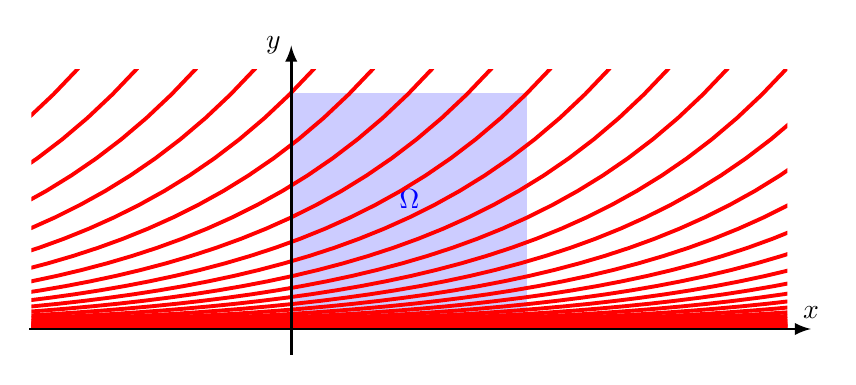
\begin{tikzpicture}[>=latex,scale=3]
\fill[color=blue!20] (0,0) rectangle (1,1);
\node[color=blue] at (0.5,0.55) {$\Omega$};
\begin{scope}
\clip (-1.1,-0.1) rectangle (2.1,1.1);
\foreach \c in {-7,-6.75,...,3}{
	\draw[color=red,line width=1.4pt]
		plot[domain={-5.1-\c}:{0.1-\c},samples=50]
			({\x},{exp(\x+\c)});
}
\end{scope}
\draw[->,line width=1pt] (-1.11,0) -- (2.20,0) coordinate[label={$x$}];
\draw[->,line width=1pt] (0,-0.11) -- (0,1.2) coordinate[label={left:$y$}];
\end{tikzpicture}
\caption{The curves $y=e^{x-c}$ used to answer the question
from which parts of the boundary the whole domain $\Omega$
can be covered.
\label{30000031:fig}}
\end{figure}
The curves are shown in figure~\ref{30000031:fig}.
\begin{teilaufgaben}
\item
Every point $(x,y)$ is covered by a curve, which can be seen as follows.
Taking the logarithm of $y=e^{x-c}$ gives $\log y = x-c$ and solving for
$c$ gives $c=x-\log y$.
\item
Only points below the exponential curve through $(1,1)$ are reachable
from the boundary.
That curve is $y=e^{x-1}$, so only points
\[
\{ (x,y) \mid y < e^{x-1} \}
\]
are reachable.
\item
Since the curves $e^{x-c}>0$ are always positive, no curve goes through
the bottom boundary.
\item
Only points above the curve through $(1,1)$ are reachable, i.~e.
\[
\{ (x,y) \mid y > e^{x-1} \}
\]
\end{teilaufgaben}
\end{loesung}
